\documentclass[a4paper,12pt,oneside]{scrbook}
\KOMAoptions{
    chapterprefix=true,
    parskip=half,
    % captions=tableheading,
    draft=false
}

% % Activar números de línea
% \usepackage{lineno}
% \linenumbers
% \setlength\linenumbersep{5pt}
% \renewcommand\linenumberfont{\normalfont\tiny\sffamily\color{gray}}

\usepackage[spanish,es-ucroman,es-noenumerate,es-tabla]{babel}
\usepackage[hidelinks]{hyperref}

\renewcommand{\listtablename}{Índice de tablas}    
\renewcommand{\listfigurename}{Índice de figuras}
\addto\extrasspanish{
    \renewcommand{\sectionautorefname}{Apartado}
    \renewcommand{\subsectionautorefname}{Apartado}
    \renewcommand{\subsubsectionautorefname}{Apartado}
}

% Márgenes del documento
\usepackage{geometry}
\geometry{left=2cm, right=2cm, top=2cm, bottom=3.3cm}

% % Interlineado 1.5
% \onehalfspacing

% Sangría 
% Ojo, la guía de KOMA-Script sugiere usar espaciado o sangría para delimitar los párrafos,
% pero no ambas cosas porque es redundante.
\setlength{\parindent}{0.5cm}

% Configuración de fuentes
\usepackage{fontspec}
\usepackage{amsmath}
\usepackage{unicode-math}   % Incluye Latin Modern Math

\setmainfont[Ligatures=TeX]{Latin Modern Sans}
\setsansfont[Ligatures=TeX]{Latin Modern Sans}
\setmonofont[Scale=MatchLowercase]{Source Code Pro}
\setmathfont{Latin Modern Math}

% Bibliografía
\usepackage{csquotes}
% APA
\usepackage[style=apa,sorting=ynt,backend=biber]{biblatex}
% % Numérica
% \usepackage[style=numeric-comp,sorting=none,backend=biber]{biblatex}
\bibliography{references}

\usepackage{array} 
\usepackage{booktabs}
\usepackage{caption}
\usepackage{enumitem}
\usepackage{float}
\usepackage{gensymb}
\usepackage{graphicx}
\usepackage{lipsum}
\usepackage{longtable}
\usepackage{microtype}
\usepackage{pdflscape}
\usepackage{rotating}
\usepackage{subcaption}
\usepackage{tabularx}
\usepackage[table]{xcolor}

% Código con coloreado de sintaxis
\usepackage{scrhack}            % Para evitar un warning sobre \float@addtolist
\usepackage{listings}
\definecolor{bluekeywords}{rgb}{0.13,0.13,1}
\definecolor{greencomments}{rgb}{0,0.5,0}
\definecolor{redstrings}{rgb}{0.9,0,0}
\definecolor{punct}{rgb}{0.1,0.1,0.55}
\definecolor{delim}{rgb}{0.1,0.1,0.55}
\definecolor{numb}{rgb}{0.65,0.16,0.16}

\lstset{
  basicstyle=\ttfamily\footnotesize,  % el estilo de la fuente usado para el código
  numbers=left,                       % donde poner los números de línea
  numberstyle=\tiny\color{gray},      % el estilo de los números de línea
  stepnumber=1,                       % el intervalo entre los números de línea
  numbersep=8pt,                      % cuánto espacio hay entre los números de línea y el código
  backgroundcolor=\color{white},      % el color de fondo de los cuadros de código
  showspaces=false,                   % muestra espacios agregando subrayado
  showstringspaces=false,             % subraya solo los espacios en las cadenas
  showtabs=false,                     % muestra tabulaciones agregando subrayado
  frame=leftline,                     % añade un marco alrededor del código
  rulecolor=\color{lightgray},        % si no se establece, el color del marco puede cambiar en los cuadros roto
  tabsize=2,                          % establece el tamaño de la tabulación
  captionpos=b,                       % establece la posición de la leyenda del cuadro de código
  breaklines=true,                    % líneas de ajuste automático
  breakatwhitespace=true,             % corta las líneas solo en los espacios en blanco
  keywordstyle=\color{bluekeywords}\bfseries,  % estilo para las palabras clave
  commentstyle=\color{greencomments}, % estilo para los comentarios
  stringstyle=\color{redstrings},     % estilo para las cadenas
  title=\lstname,                     % muestra el nombre de los archivos listados
  literate=
     *{0}{{{\color{numb}0}}}{1}
      {1}{{{\color{numb}1}}}{1}
      {2}{{{\color{numb}2}}}{1}
      {3}{{{\color{numb}3}}}{1}
      {4}{{{\color{numb}4}}}{1}
      {5}{{{\color{numb}5}}}{1}
      {6}{{{\color{numb}6}}}{1}
      {7}{{{\color{numb}7}}}{1}
      {8}{{{\color{numb}8}}}{1}
      {9}{{{\color{numb}9}}}{1}
      {:}{{{\color{punct}{:}}}}{1}
      {,}{{{\color{punct}{,}}}}{1}
      {\{}{{{\color{delim}{\{}}}}{1}
      {\}}{{{\color{delim}{\}}}}}{1}
      {[}{{{\color{delim}{[}}}}{1}
      {]}{{{\color{delim}{]}}}}{1},
}

%% JavaScript
% https://github.com/ghammock/LaTeX_Listings_JavaScript_ES6
\lstdefinelanguage{JavaScript}{
  morekeywords=[1]{break, continue, delete, else, for, function, if, in,
    new, return, this, typeof, var, void, while, with},
  % Literals, primitive types, and reference types.
  morekeywords=[2]{false, null, true, boolean, number, undefined,
    Array, Boolean, Date, Math, Number, String, Object},
  % Built-ins.
  morekeywords=[3]{eval, parseInt, parseFloat, escape, unescape},
  sensitive,
  morecomment=[s]{/*}{*/},
  morecomment=[l]//,
  morecomment=[s]{/**}{*/}, % JavaDoc style comments
  morestring=[b]',
  morestring=[b]"
}[keywords, comments, strings]

\lstalias[]{ES6}[ECMAScript2015]{JavaScript}

\lstdefinelanguage[ECMAScript2015]{JavaScript}[]{JavaScript}{
  morekeywords=[1]{await, async, case, catch, class, const, default, do,
    enum, export, extends, finally, from, implements, import, instanceof,
    let, static, super, switch, throw, try},
  morestring=[b]` % Interpolation strings.
}          % Estilo y definiciones para lenguajes adicionales

% Descripción de algoritmos
\usepackage[
    ruled,              % Dibuja una línea horizontal sobre y bajo el bloque del algoritmo
    vlined,             % Dibuja líneas verticales al inicio y al final de los bloques de control (if-else, while, for, etc.)
    commentsnumbered,   % Numera los comentarios dentro del algoritmo
    linesnumbered,      % Numera cada línea del algoritmo
    inoutnumbered,      % Numera las líneas de entrada y salida
    titlenotnumbered,   % No numera el título del algoritmo
    noend               % Omite los comandos 'end' (\EndWhile, \EndFor, \EndIf, etc.)
]{algorithm2e}
%% Definición de la estructura Do..while
% \Do{this end condition}{
%     do these things\;
% }
\SetKwRepeat{Do}{do}{while}

\newenvironment{abstract}[1][\abstractname]{
    \cleardoublepageusingstyle{empty}
    \thispagestyle{empty}
    \begin{center}\textbf{#1}\end{center}
    \begin{itshape}\par\noindent%
}
{\end{itshape}}

\newenvironment{keywords}[1][Keywords]
{\vspace{7pt}\par\noindent\textup{\textbf{#1: }}\begin{upshape}}
{\end{upshape}}

% Formato de capítulos
% Eliminar el punto y reducir el espacio entre el prefijo y el nombre del capítulo 
\renewcommand*{\chapterformat}{%
    \mbox{\chapappifchapterprefix{\nobreakspace}\thechapter
    \IfUsePrefixLine{}{\enskip}}}
\renewcommand{\chapterheadmidvskip}{\vskip 0pt}

% Redefinición de las entradas de los capítulos en la tabla de contenidos
% para que aparezca el prefijo.
\let\originaladdchaptertocentry\addchaptertocentry
\renewcommand*{\addchaptertocentry}[2]{%
  \IfArgIsEmpty{#1}{% Entrada sin número
    \originaladdchaptertocentry{#1}{#2}%
  }{% Entrada con número
    % Eliminar el número y poner el prefijo directamente en el título del capítulo
    \originaladdchaptertocentry{}{\chapapp~#1\autodot\space#2}%
  }%
}

\begin{document}   

%%%%%%%%%%%%%%%%%%%%%%%%%%%%%%%%%%%%%%%%%%%%%%%%%%%%%%%%%%%%%%%%%%%%%%%%%%%%%%%
% Portada y metadatos
%%%%%%%%%%%%%%%%%%%%%%%%%%%%%%%%%%%%%%%%%%%%%%%%%%%%%%%%%%%%%%%%%%%%%%%%%%%%%%%

% Metadatos del PDF
\hypersetup{
    pdftitle='Título del trabajo',
    pdfauthor='Nombre y Apellidos',
    pdfsubject={Trabajo de Fin de Grado},
}

\pagestyle{empty}
\newcommand{\HRule}{\rule{\linewidth}{0.3mm}}
{
    \setlength{\parindent}{0mm}
    \setlength{\parskip}{0mm}
    
    \vspace*{1.20cm}
    
\includegraphics[width=9.81cm]{images/logos/escuela-ingenieria-tecnologia-original}
    \vspace*{\stretch{0.9}}
    
    {\centering
    \fontsize{32pt}{32pt}\selectfont Trabajo de Fin de Grado\\[10pt]
    \fontsize{20pt}{20pt}\selectfont Grado en Ingeniería Informática\par}
    \HRule\vspace*{2mm}
    \begin{flushright}
            {\fontsize{32pt}{32pt}\selectfont Título del trabajo} \\[3mm]
            {\fontsize{18pt}{18pt}\selectfont \textit{Title in English}} \\[11mm]
            {\fontsize{16pt}{16pt}\selectfont Nombre y Apellidos}
    \end{flushright}\vspace*{12mm}
    \HRule
    
    \vspace*{\stretch{1}}
    \begin{center}
        \fontsize{18pt}{18pt}\selectfont La Laguna, \today
    \end{center}
}

%%%%%%%%%%%%%%%%%%%%%%%%%%%%%%%%%%%%%%%%%%%%%%%%%%%%%%%%%%
% Certificado
%%%%%%%%%%%%%%%%%%%%%%%%%%%%%%%%%%%%%%%%%%%%%%%%%%%%%%%%%%
\frontmatter
\cleardoublepageusingstyle{empty}
\thispagestyle{empty}

{
\setlength\parindent{0pt}
    D. \textbf{Nombre Apellido1 Apellido2}, profesor Titular de Universidad adscrito al Departamento de Nombre del Departamento de la Universidad de La Laguna, como tutor
    
    \bigskip
    D. \textbf{Nombre Apellido1 Apellido2}, profesor Titular de Universidad adscrito al Departamento de Nombre del Departamento de la Universidad de La Laguna, como cotutor\pagestyle{empty}
    
    \bigskip
    \bigskip
    \textbf{C E R T I F I C A (N)}

    \bigskip
    Que la presente memoria titulada:
    
    \bigskip
    \begin{quote}
    \textit{``Título del Trabajo''}
    \end{quote}
    
    \bigskip
    \noindent ha sido realizada bajo su dirección por D. \textbf{Nombre Apellido1 Apellido2}.
    
    \bigskip
    Y para que así conste, en cumplimiento de la legislación vigente y a los efectos
    oportunos, firman la presente en La Laguna a \today
}

%%%%%%%%%%%%%%%%%%%%%%%%%%%%%%%%%%%%%%%%%%%%%%%%%%%%%%%%%%
% Agradecimientos
%%%%%%%%%%%%%%%%%%%%%%%%%%%%%%%%%%%%%%%%%%%%%%%%%%%%%%%%%%
\cleardoublepageusingstyle{empty}
\thispagestyle{empty}

\begin{flushright}
    \setlength{\parindent}{0mm}

    {\LARGE Agradecimientos}
    \vspace{8mm}
    
    \begin{large}
    XXX
    
    XXX
    
    XXX
    
    XXX
    
    \end{large}
\end{flushright}

%%%%%%%%%%%%%%%%%%%%%%%%%%%%%%%%%%%%%%%%%%%%%%%%%%%%%%%%%%
% Licencia
%%%%%%%%%%%%%%%%%%%%%%%%%%%%%%%%%%%%%%%%%%%%%%%%%%%%%%%%%%
\cleardoublepageusingstyle{empty}
\thispagestyle{empty}

{\noindent\LARGE Licencia}

\textcolor{red}{Elige una licencia y elimina el testo de opciones.}

\bigskip
\textcolor{red}{• Si NO quiere permitir que se compartan las adaptaciones de tu obra y NO quieres permitir usos comerciales de tu obra, indica:}

\begin{center}
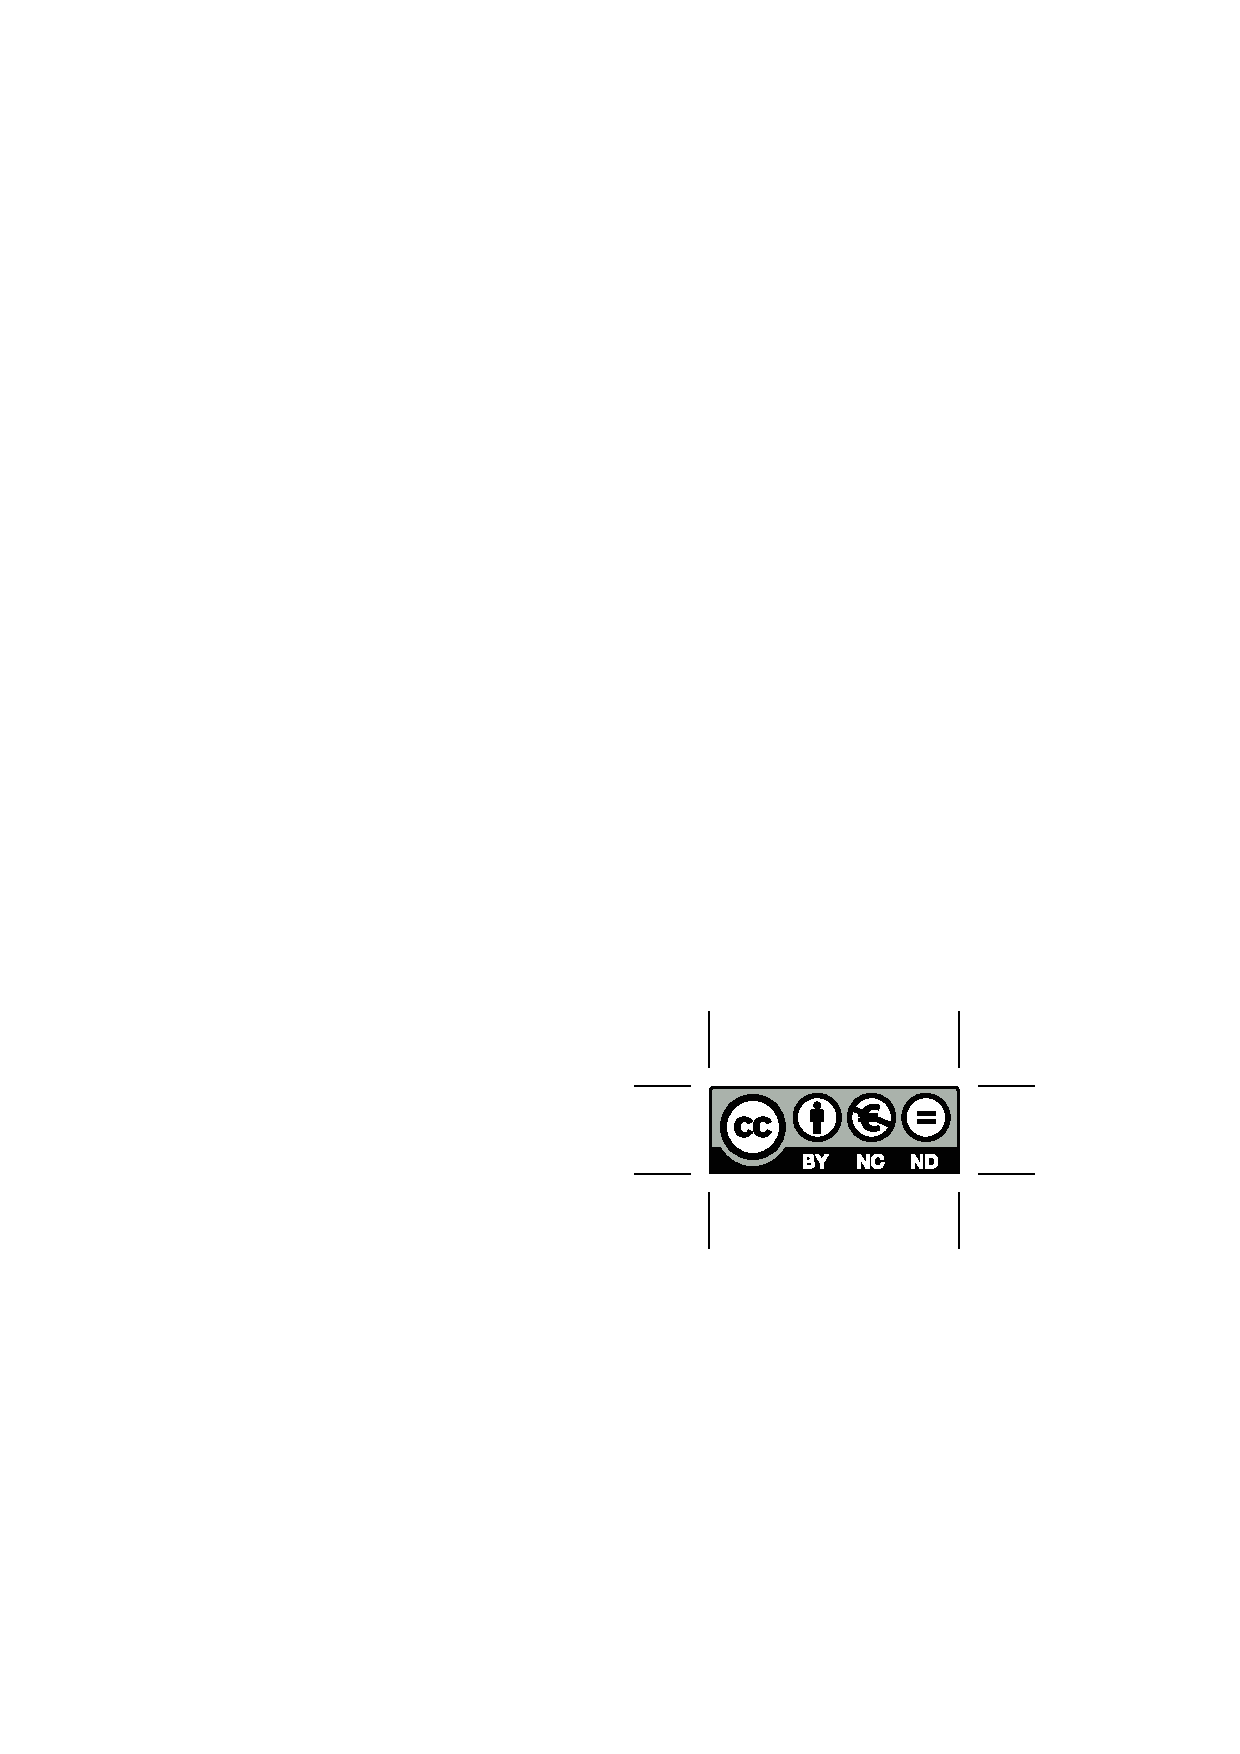
\includegraphics[width=4.66cm]{images/licenses/by-nc-nd.eu}
\end{center}

\begin{large}
© Esta obra está bajo una licencia de Creative Commons Reconocimiento-NoComercial-SinObraDerivada 4.0 Internacional.
\end{large}

\bigskip
\bigskip
\bigskip
\textcolor{red}{• Si quiere permitir que se compartan las adaptaciones de tu obra mientras se comparta de la misma manera y NO quieres permitir usos comerciales de tu obra, indica:}

\begin{center}
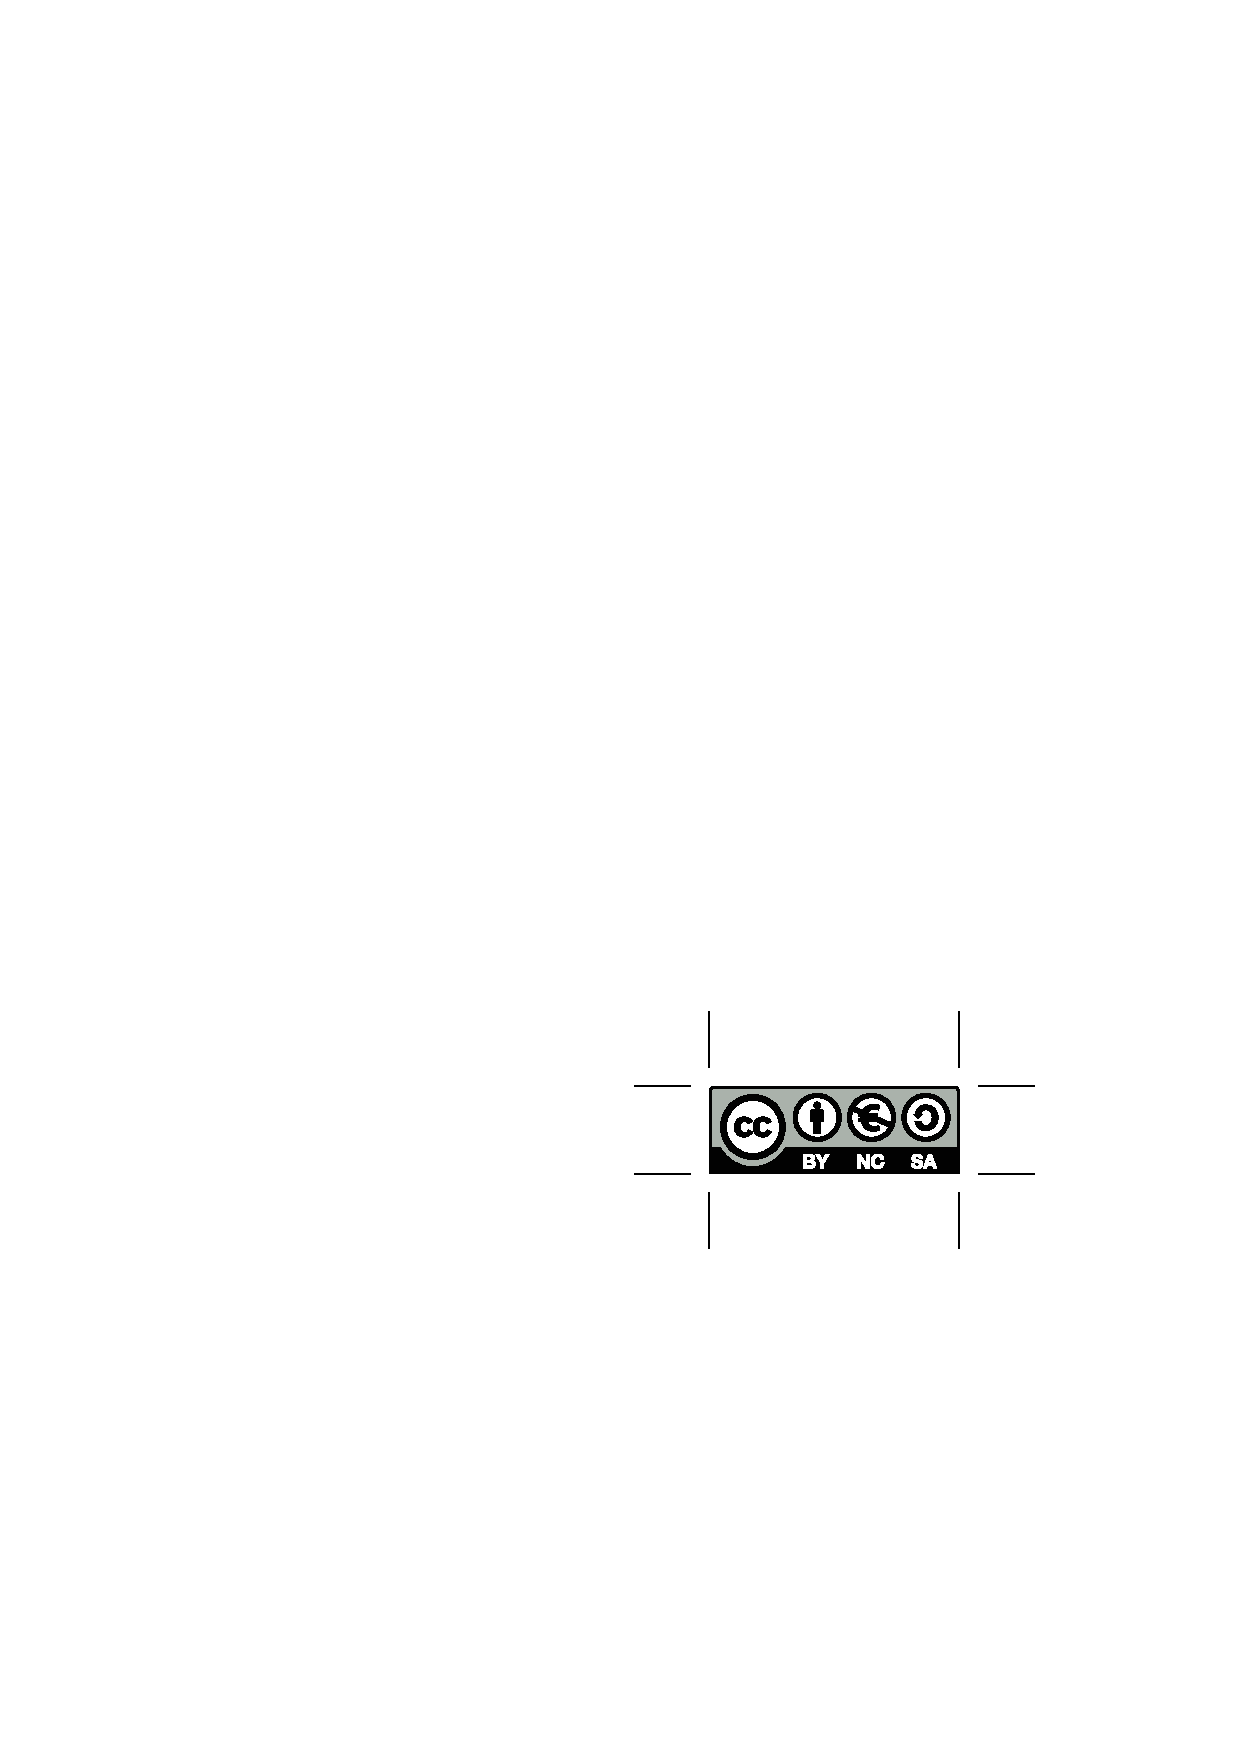
\includegraphics[width=4.66cm]{images/licenses/by-nc-sa.eu}
\end{center}

\begin{large}
© Esta obra está bajo una licencia de Creative Commons Reconocimiento-NoComercial-CompartirIgual 4.0 Internacional.
\end{large}

\bigskip
\bigskip
\bigskip
\textcolor{red}{• Si quiere permitir que se compartan las adaptaciones de tu obra y NO quieres permitir usos comerciales de tu obra, indica:}

\begin{center}
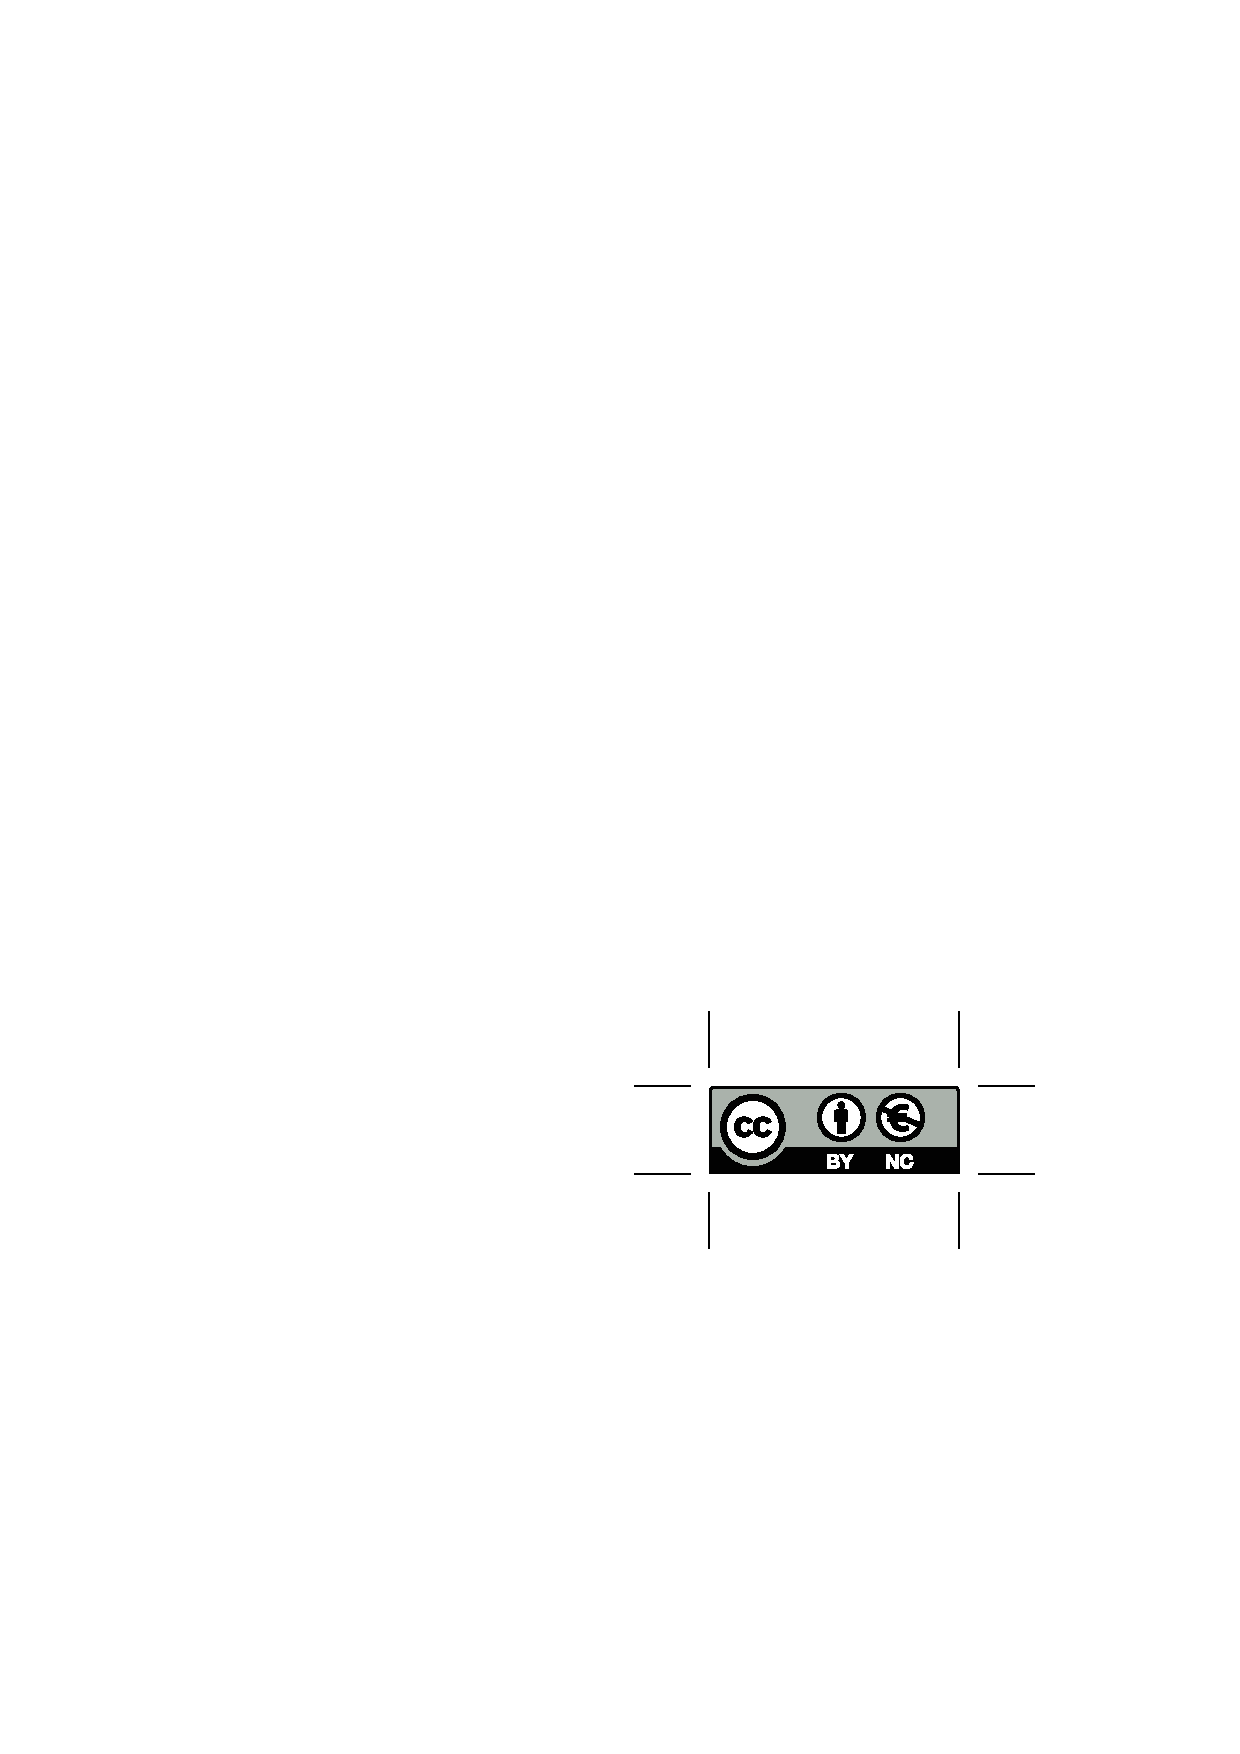
\includegraphics[width=4.66cm]{images/licenses/by-nc.eu}
\end{center}

\begin{large}
© Esta obra está bajo una licencia de Creative Commons Reconocimiento-NoComercial 4.0 Internacional.
\end{large}

\bigskip
\bigskip
\bigskip
\textcolor{red}{• Si NO quiere permitir que se compartan las adaptaciones de tu obra y quieres permitir usos comerciales de tu obra, indica:}

\begin{center}
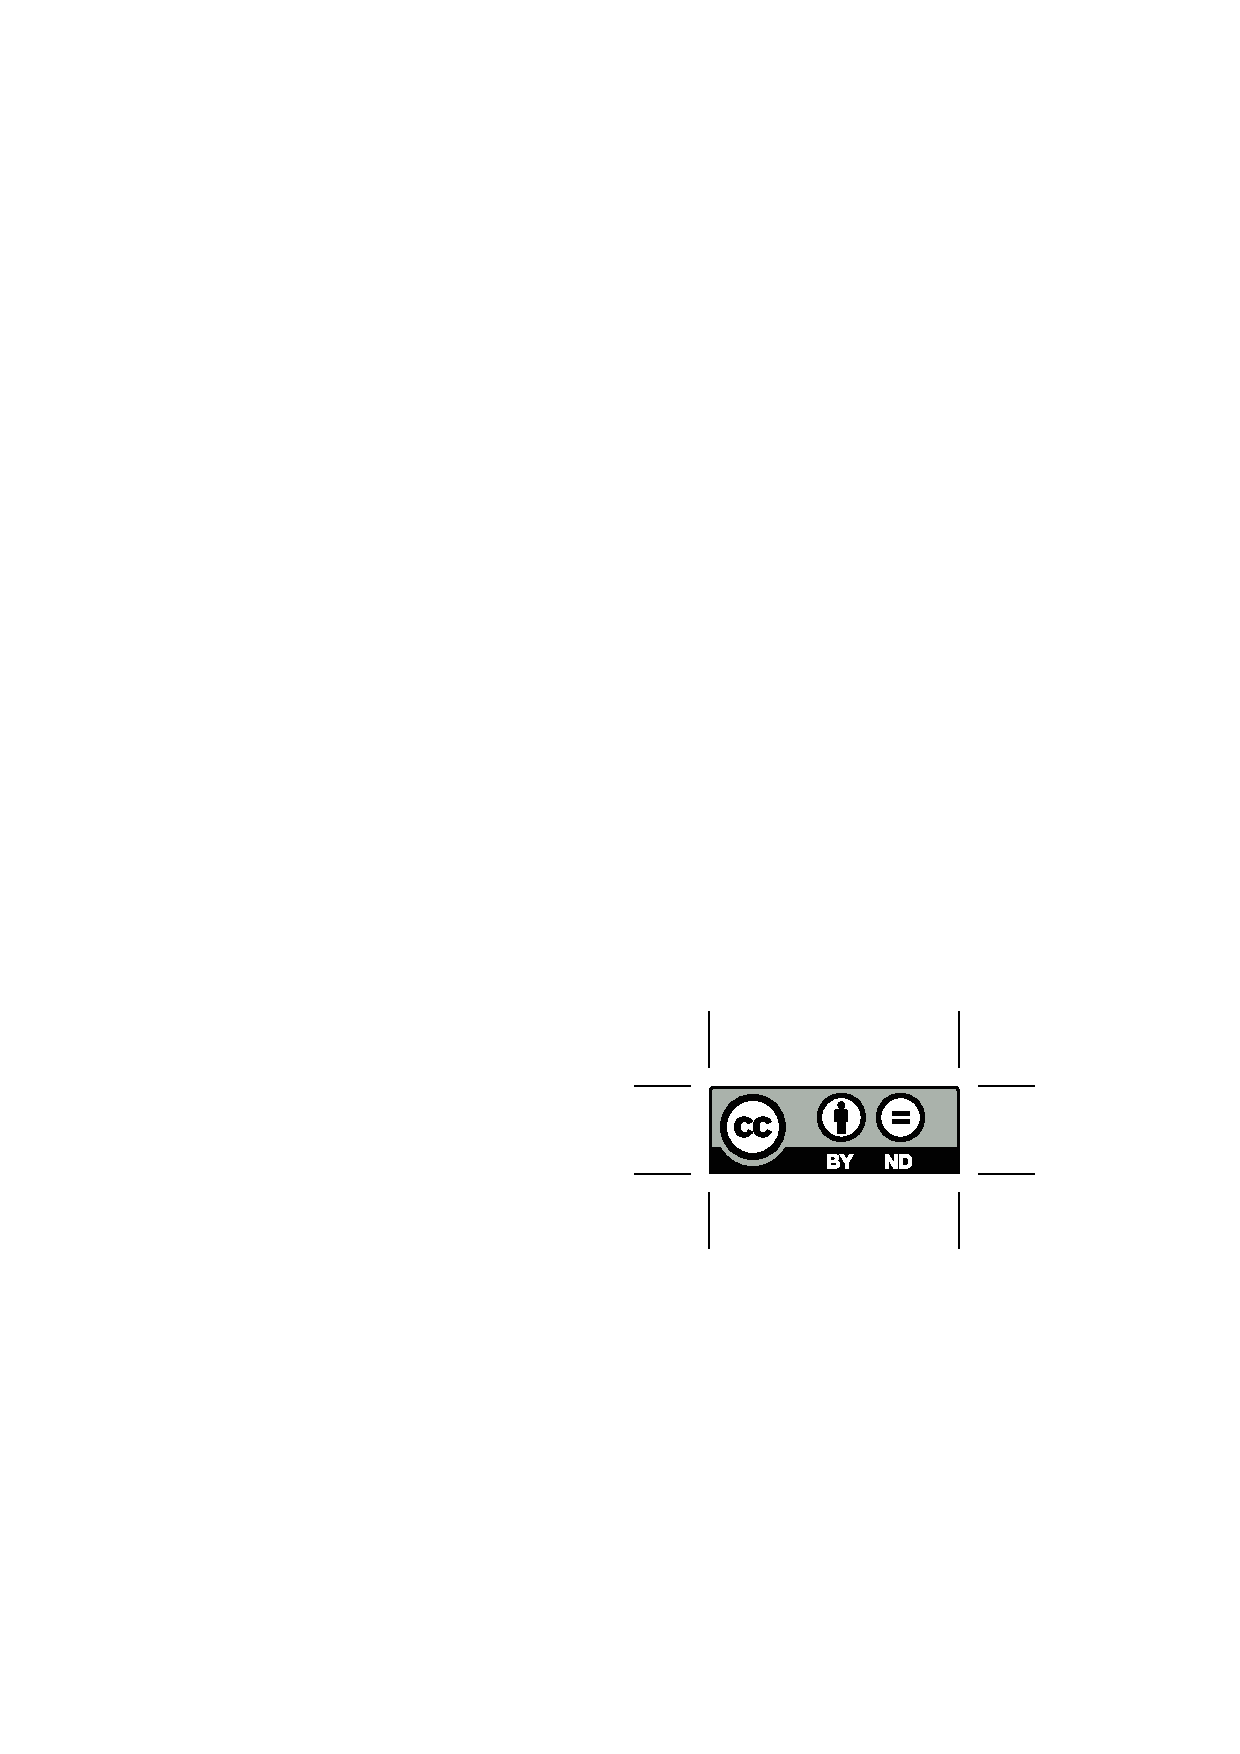
\includegraphics[width=4.66cm]{images/licenses/by-nd}
\end{center}

\begin{large}
© Esta obra está bajo una licencia de Creative Commons Reconocimiento-SinObraDerivada 4.0 Internacional.
\end{large}

\bigskip
\bigskip
\bigskip
\textcolor{red}{• Si quiere permitir que se compartan las adaptaciones de tu obra mientras se comparta de la misma manera y quieres permitir usos comerciales de tu obra (licencia de Cultura Libre) indica:}

\begin{center}
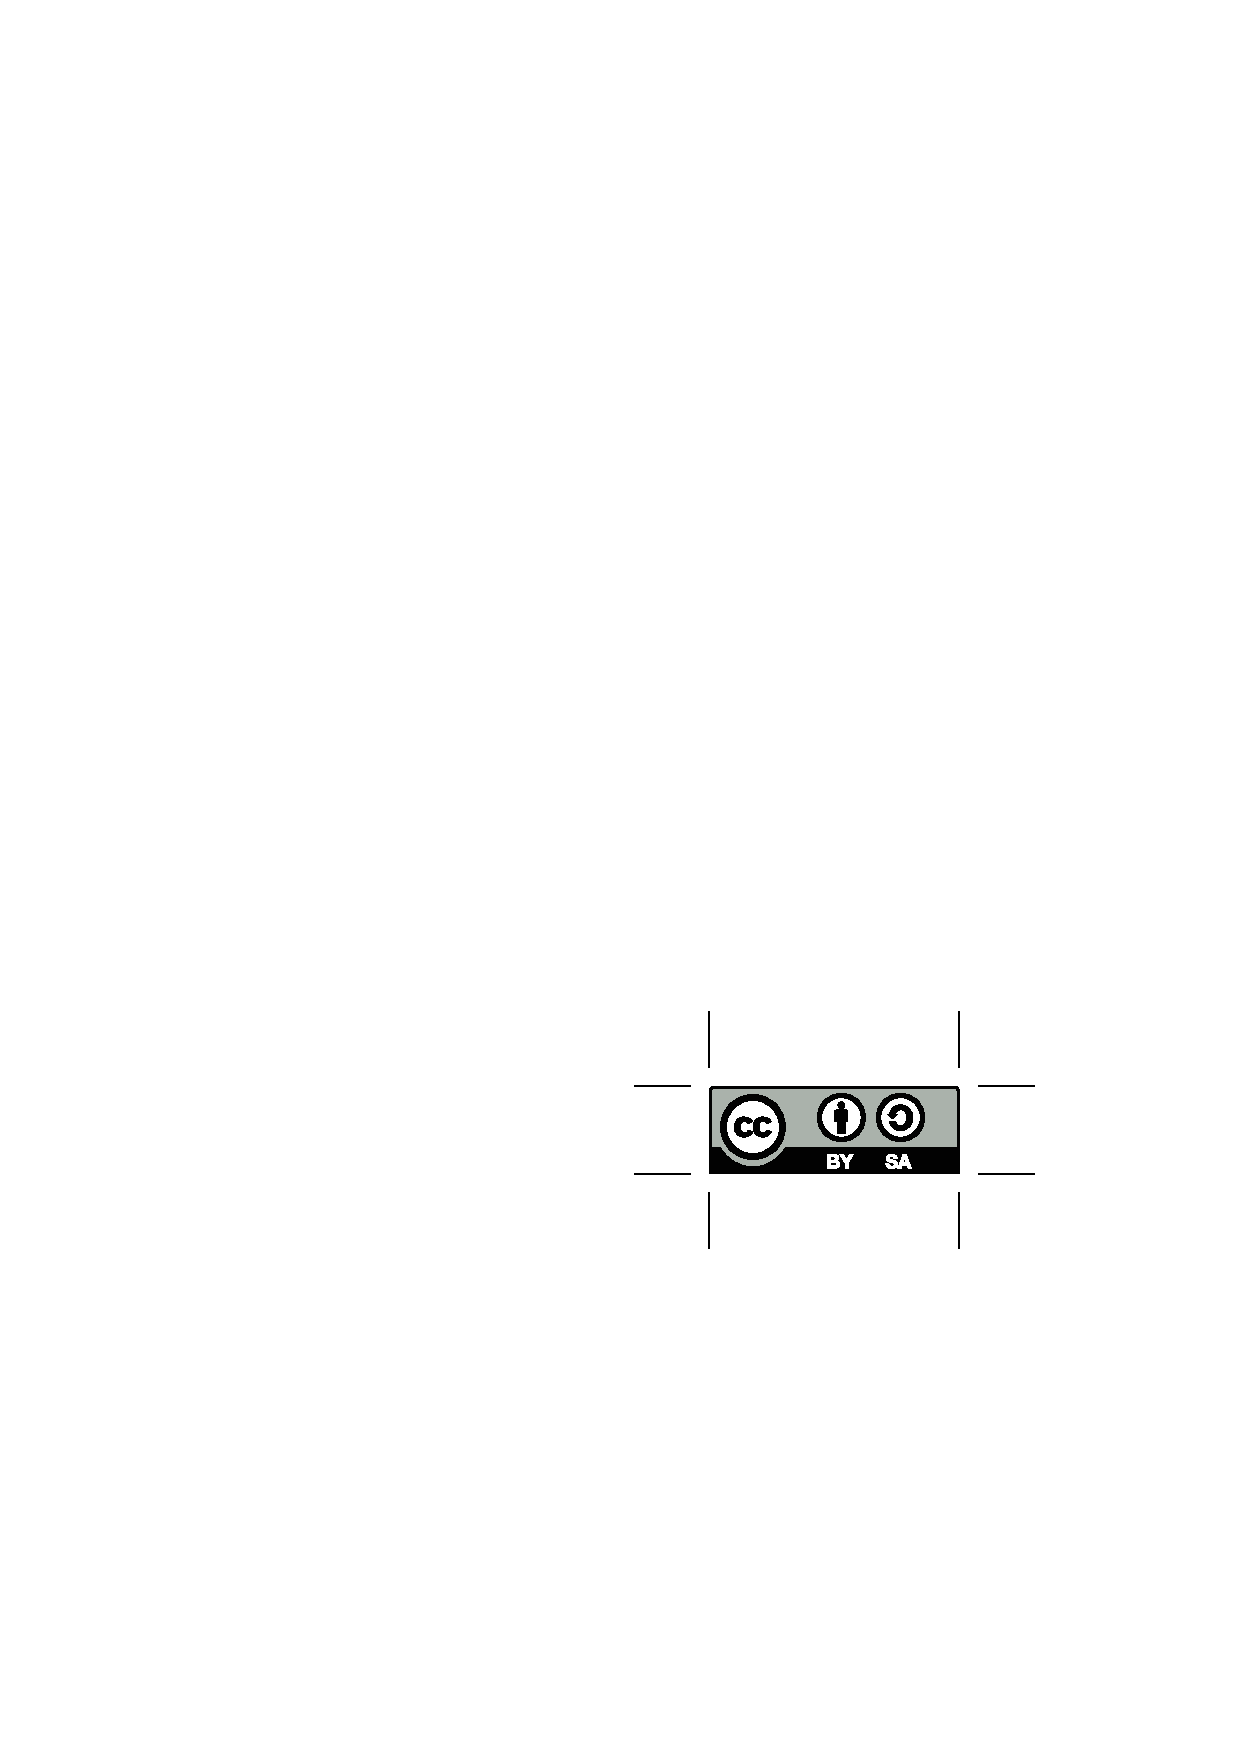
\includegraphics[width=4.66cm]{images/licenses/by-sa}
\end{center}

\begin{large}
© Esta obra está bajo una licencia de Creative Commons Reconocimiento-CompartirIgual 4.0 Internacional.
\end{large}

\bigskip
\bigskip
\bigskip
\textcolor{red}{• Si quiere permitir que se compartan las adaptaciones de tu obra y quieres permitir usos comerciales de tu obra (licencia de Cultura Libre) indica:}

\begin{center}
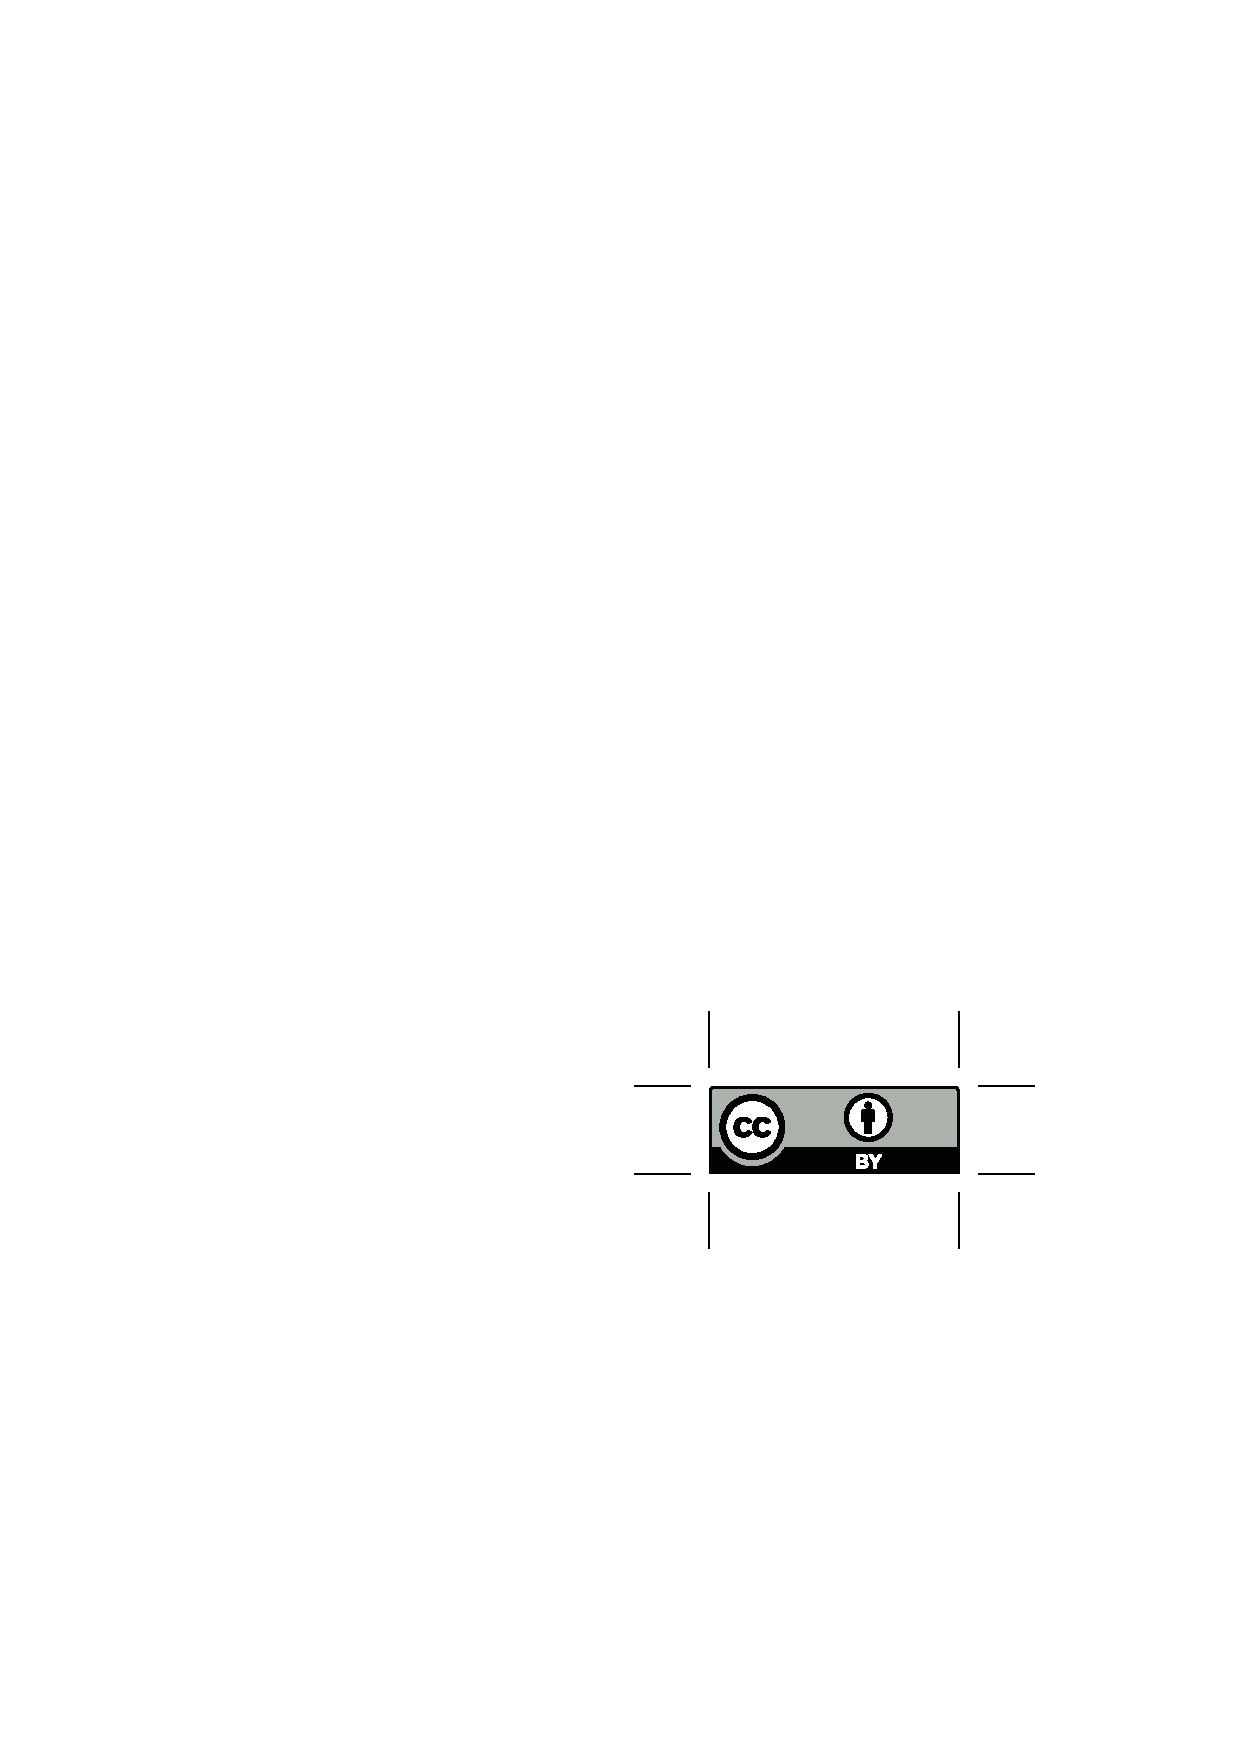
\includegraphics[width=4.66cm]{images/licenses/by}
\end{center}

\begin{large}
© Esta obra está bajo una licencia de Creative Commons Reconocimiento 4.0 Internacional.
\end{large}

%%%%%%%%%%%%%%%%%%%%%%%%%%%%%%%%%%%%%%%%%%%%%%%%%%%%%%%%%%
% Resumen
%%%%%%%%%%%%%%%%%%%%%%%%%%%%%%%%%%%%%%%%%%%%%%%%%%%%%%%%%%
\begin{abstract}
El objetivo de este trabajo ha sido.... bla, bla, bla, bla, bla, bla, bla, bla, bla...

La competencia [E6], que figura en la guía docente, indica que en la memoria del trabajo se ha de incluir: antecedentes, problemática o estado del arte, objetivos, fases y desarrollo del proyecto, conclusiones, y líneas futuras.

Se ha incluido el apartado de 'Licencia' con todas las posibles licencias abiertas (Creative Commons). En el caso en que se decida hacer público el contenido de la memoria, habrá que elegir una de ellas (y borrar las demás). La decisión de hacer pública o no la memoria se indica en el momento de subir la memoria a la Sede Electrónica de la ULL, paso necesario en el proceso de presentación del TFG.

El documento de memoria debe tener un máximo de 50 páginas.

No se deben dejar páginas en blanco al comenzar un capítulo, ya que el documento no está pensado para ser impreso sino visionado con un lector de PDF.

También es recomendable usar márgenes pequeños, ya que, al firmar digitalmente por la Sede Electrónica, se coloca un marco alrededor del texto original.

El tipo de letra base ha de ser de 12 ptos.

\begin{keywords}[Palabras clave]
Palabra reservada1, Palabra reservada2,...
\end{keywords}
\end{abstract}

%%%%%%%%%%%%%%%%%%%%%%%%%%%%%%%%%%%%%%%%%%%%%%%%%%%%%%%%%
\cleardoublepageusingstyle{empty}
\thispagestyle{empty}

\begin{abstract}[Abstract]
Here should be the abstract in a foreing language...

\begin {keywords}
Keyword1, Keyword2, Keyword3,...
\end{keywords}
\end{abstract}

%%%%%%%%%%%%%%%%%%%%%%%%%%%%%%%%%%%%%%%%%%%%%%%%%%%%%%%%%
\pagestyle{plain}
\cleardoublepage
\setcounter{page}{1} 

\tableofcontents
\listoffigures
\listoftables

%%%%%%%%%%%%%%%%%%%%%%%%%%%%%%%%%%%%%%%%%%%%%%%%%%%%%%%%%%
% Contenidos
%%%%%%%%%%%%%%%%%%%%%%%%%%%%%%%%%%%%%%%%%%%%%%%%%%%%%%%%%%
\mainmatter

\chapter{Introducción}
\label{ch:intro}

\noindent Cualquier capítulo puede tener múltiples apartados, como el \autoref{sec:apartado1} o el \autoref{sec:sección2} de este mismo capítulo.

También está el \autoref{sec:ch2_1} del \autoref{ch:dos} que tiene la \autoref{fig:other}.

Es buena idea usar \verb|\noindent| al principio del primer párrafo, tras el encabezado de una sección o capítulo, para desactivar la sangría temporalmente.

\section{Listas de elementos}
\label{sec:apartado1}

\noindent Esta la lista de elementos del \autoref{sec:apartado1}:

\begin{itemize}
    \item Item 1
    \begin{itemize}
        \item Item 1
        \item Item 2
        \item Item 3
        \item Item 4
    \end{itemize}
    
    \item Item 2
    \item Item 3
    \item Item 4
\end{itemize}

\section{Enumeraciones}
\label{sec:sección2}

\noindent Esto es una lista enumerada, que puede estar relacionada con la \autoref{fig:intro}

\begin{enumerate}
    \item Item 1
    \begin{enumerate}
        \item Item 1
        \item Item 2
        \item Item 3
    \end{enumerate}
    \item Item 2
    \item Item 3
\end{enumerate}

\section{Figuras y tablas}

\noindent En la \autoref{fig:intro} se puede ver una figura de ejemplo. Las tablas, las figuras y los algoritmos (ver el \autoref{Apendice1:ZZZ}) son flotantes. Esto quiere decir que \LaTeX{} los intentará ubicar en el mejor lugar posible al componer el documento, intentando respetar ciertas reglas tipográficas. Como este lugar puede ser diferente a la posición que realmente ocupan en el texto, \textbf{es importante referenciar en el texto todas las figuras y las tablas}, en los diferentes puntos donde se hable de ellas.

\begin{figure}[htbp]
   \centering
   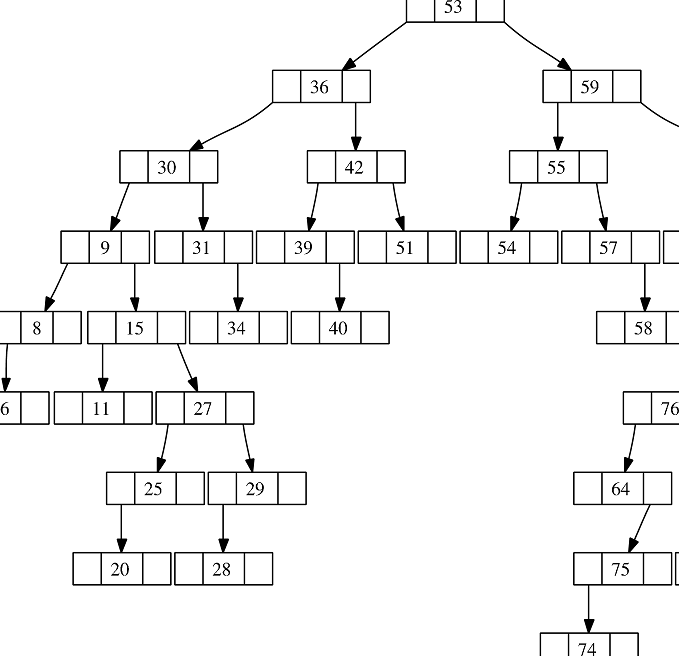
\includegraphics[width=0.8\linewidth]{images/figura_1}
   \caption{Ejemplo de figura.}
   \label{fig:intro}
\end{figure}

La \autoref{tbl:presupuesto} en el \autoref{ch:presupuesto} es un ejemplo de tabla hecha con el paquete \verb|tabularx|.

Al crear tablas, figuras u otros elementos flotantes es aconsejable indicar siempre los especificadores de ubicación \verb|[htbp]|, tal y como se hace en los ejemplos de esta plantilla. De esta forma \LaTeX{} intentará primero ponerlos en el lugar; si no puede, intentará ponerlos en la parte superior o inferior de la misma página y, en caso extremo, los pondrá en páginas especiales que solo contienen flotantes.

No es buena idea usar especificadores como \verb|[!h]| o \verb|[H]| para forzar una ubicación determinada. El motivo es que eso impide a \LaTeX{} buscar la mejor forma de componer el documento, pudiendo dar como resultado páginas que se ven muy raras --por ejemplo, dejando muchos huecos libres entre el texto--.
Solo se deben utilizar estos especificadores cuando es absolutamente necesario, como ocurre en el \autoref{ch:presupuesto}, donde interesa que las tablas del presupuesto aparezca juntas, en la posición preestablecida.

\section{Código y algoritmos}

\noindent En el \autoref{apx:1} se pueden observar varios ejemplos de entornos para describir algoritmos y código.

\section{Citas}

\noindent Las referencias bibliográficas se deben indicar en el archivo \texttt{references.bib} y se citan en el texto. Las referencias no citadas no aparecerán en el apartado de la bibliografía.

Las citas pueden ser entre paréntesis \parencite{examplearticle} o \emph{en línea}, como la de \cite{examplegithub}.

Las  reglas para citar \parencite{ulllibguide} permiten citar cualquier cosa: artículos de investigación, libros, entradas de la Wikipedia, blogs, vídeos de Youtube o repositorios de GitHub, entre otros. 

En el \autoref{ch:cuatro} se puede ver otro tipo de citas, usando el paquete \texttt{csquotes}, donde se traslada de forma literal una porción del texto original al documento.
 
\section{Otra sección...}

\noindent \lipsum[1]

\subsection{Con subsección...}

\noindent \lipsum[2]
\chapter{Título del Capítulo 2}
\label{ch:dos}

\noindent Los capítulos intermedios servían para cubrir los siguientes aspectos: antecedentes, problemática o estado del arte, objetivos, fases y desarrollo del proyecto.

En el capítulo anterior se ha introducido la \autoref{fig:intro} y en este la \autoref{fig:other}. 

\section{Primera sección de otro capítulo}
\label{sec:ch2_1}

\begin{figure}[htb]
   \centering
   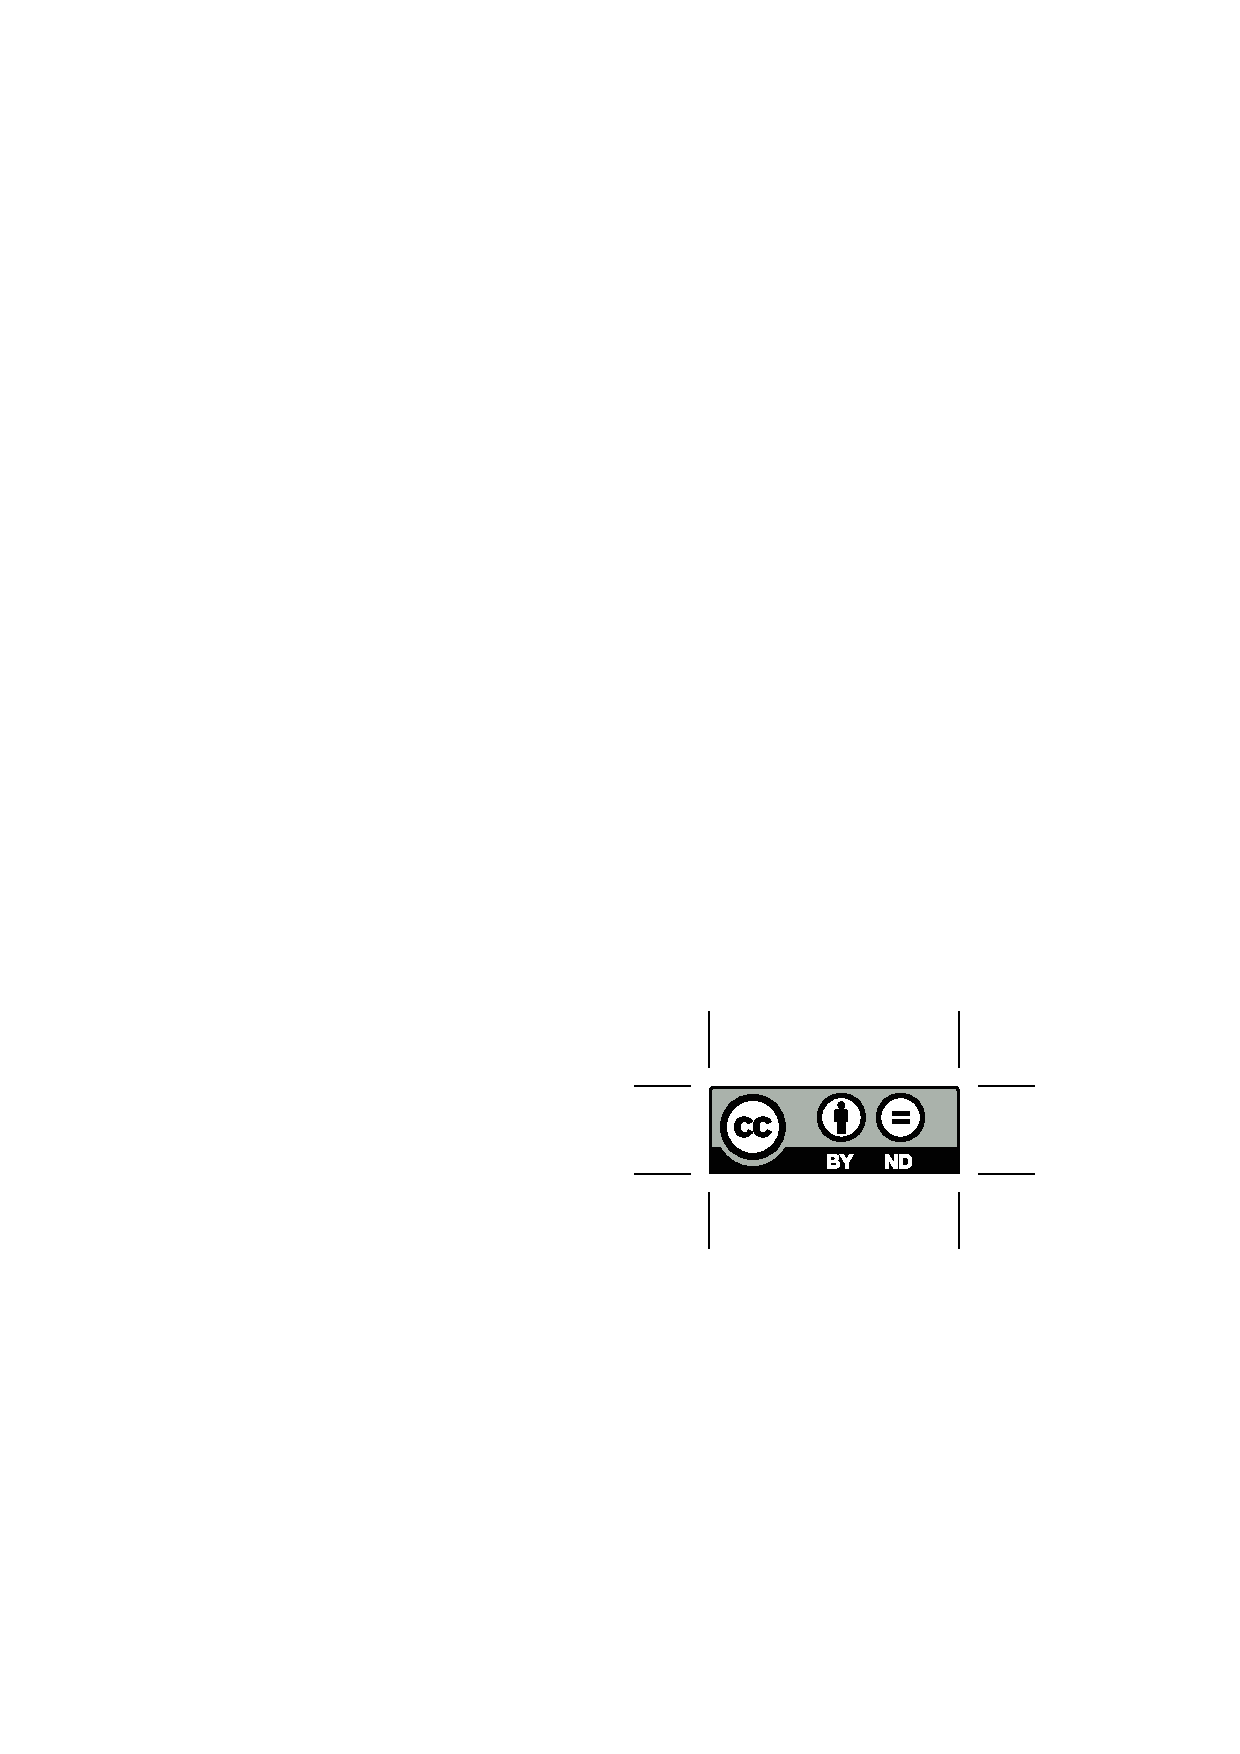
\includegraphics[width=0.5\linewidth]{images/licenses/by-nd}
   \caption{Otra figura.}
   \label{fig:other}
\end{figure}

\lipsum[3]

\section{Segunda sección de otro capítulo}

\noindent \lipsum[4-5]



\chapter{Título del Capítulo 3}
\label{ch:tres}

\noindent Los capítulos intermedios servirán para cubrir los siguientes aspectos: antecedentes, problemática o estado del arte, objetivos, fases y desarrollo del proyecto.

Bla, Bla, Bla, .....

\section{Primera sección de este capítulo}
\section{Segundo apartado de este capítulo}
\section{Tercer apartado de este capítulo}
\chapter{Título del Capítulo 4}
\label{ch:cuatro}

\noindent Los capítulos intermedios servirán para cubrir los siguientes aspectos: antecedentes, problemática o estado del arte, objetivos, fases y desarrollo del proyecto.

El \autoref{ch:intro} se describió bla, bla, bla …
\chapter{Conclusiones y líneas futuras}
\label{ch:conclusiones}

\noindent Este capítulo es obligatorio. Toda memoria de Trabajo de Fin de Grado debe incluir unas conclusiones y unas líneas de trabajo futuro 
This chapter is compulsory. The memory should include an extended summary and conclusions in english. 
\chapter{Presupuesto}
\label{ch:presupuesto}

\noindent Este capítulo es obligatorio. Toda memoria de Trabajo de Fin de Grado debe incluir un presupuesto.

\section{Sección Uno}

\begin{table}[htb]
    \begin{center}
        \begin{tabularx}{0.8\textwidth} { X X }
            \toprule
            \textbf{Tipos} & \textbf{Descripción} \\
            \midrule
            AAAA  & BBBB \\
            CCCC  & DDDD \\
            EEEE  & FFFF \\
            GGGG  & HHHH \\
            \bottomrule
        \end{tabularx}
    \end{center}
    \caption{Resumen de tipos}
    \label{tbl:presupuesto}
\end{table}

\appendix

\section{Algoritmo XXX}
\label{Apendice1:XXX}

\begin{center}
\begin{footnotesize}
\begin{verbatim}

/***********************************************************************************
*
* Fichero .h
*
***********************************************************************************
*
* AUTORES
*   
*
* FECHA
*   
*
* DESCRIPCION
*   
*
************************************************************************************/

\end{verbatim}
\end{footnotesize}
\end{center}

\section{Algoritmo YYY}
\label{Apendice1:YYY}

\begin{center}
\begin{footnotesize}
\begin{verbatim}


/***********************************************************************************
 *
 * Fichero .h
 *
 ***********************************************************************************
 *
 * AUTORES
 *
 * FECHA
 *
 * DESCRIPCION
 *
 *
 ************************************************************************************/
 
\end{verbatim}
\end{footnotesize}
\end{center}

\section{Algoritmo ZZZ}
\label{Apendice1:ZZZ}

\begin{center}
\begin{footnotesize}
\begin{verbatim}


/***********************************************************************************
 *
 * Fichero .h
 *
 ***********************************************************************************
 *
 * AUTORES
 *
 * FECHA
 *
 * DESCRIPCION
 *
 *
 ************************************************************************************/
 
\end{verbatim}
\end{footnotesize}
\end{center}


\chapter{Título del Apéndice 2}
\label{appendix:2}

\section{Otro apéndice: Sección 1}
\lipsum[1]

\section{Otro apéndice: Sección 2}
\lipsum[2]

%%%%%%%%%%%%%%%%%%%%%%%%%%%%%%%%%%%%%%%%%%%%%%%%%%%%%%%%%%
% Bibliografía
%%%%%%%%%%%%%%%%%%%%%%%%%%%%%%%%%%%%%%%%%%%%%%%%%%%%%%%%%%
\backmatter

\printbibliography
%%%%%%%%%%%%%%%%%%%%%%%%%%%%%%%%%%%%%%%%%%%%%%%%%%%%%%%%%%

\end{document}

